\documentclass[tikz,border=8pt]{standalone}
\usepackage[T1]{fontenc}
\usepackage{helvet}
\renewcommand{\familydefault}{\sfdefault}
\usepackage{amsmath}
\usepackage{xcolor}
\usetikzlibrary{arrows.meta, positioning}

\definecolor{ink}{HTML}{1F2937}
\definecolor{blueA}{HTML}{E8F1FB}
\definecolor{blueB}{HTML}{2F6B9A}
\definecolor{tealA}{HTML}{E7F7F5}
\definecolor{tealB}{HTML}{1D8B74}
\definecolor{orangeA}{HTML}{FFF1E6}
\definecolor{orangeB}{HTML}{C86A1A}
\definecolor{greenA}{HTML}{EAF7E9}
\definecolor{greenB}{HTML}{2E7D32}
\definecolor{redA}{HTML}{FDECEC}
\definecolor{redB}{HTML}{B23A3A}
\definecolor{grayB}{HTML}{5B6470}

\tikzset{
  title/.style={font=\bfseries\fontsize{24}{26}\selectfont, text=ink},
  subtitle/.style={font=\bfseries\fontsize{15}{17}\selectfont, text=ink},
  body/.style={font=\fontsize{11}{13}\selectfont, text=ink},
  smallbody/.style={font=\fontsize{10}{12}\selectfont, text=ink},
  box/.style={rounded corners=14pt, draw=grayB!35, line width=1.1pt, fill=white, inner sep=12pt, align=left},
  bluebox/.style={box, fill=blueA},
  tealbox/.style={box, fill=tealA},
  orangebox/.style={box, fill=orangeA},
  greenbox/.style={box, fill=greenA},
  redbox/.style={box, fill=redA}
}
\newcommand{\subtitle}{\bfseries\fontsize{15}{17}\selectfont\color{ink}}
\newcommand{\body}{\fontsize{11}{13}\selectfont\color{ink}}
\newcommand{\smallbody}{\fontsize{10}{12}\selectfont\color{ink}}

\begin{document}
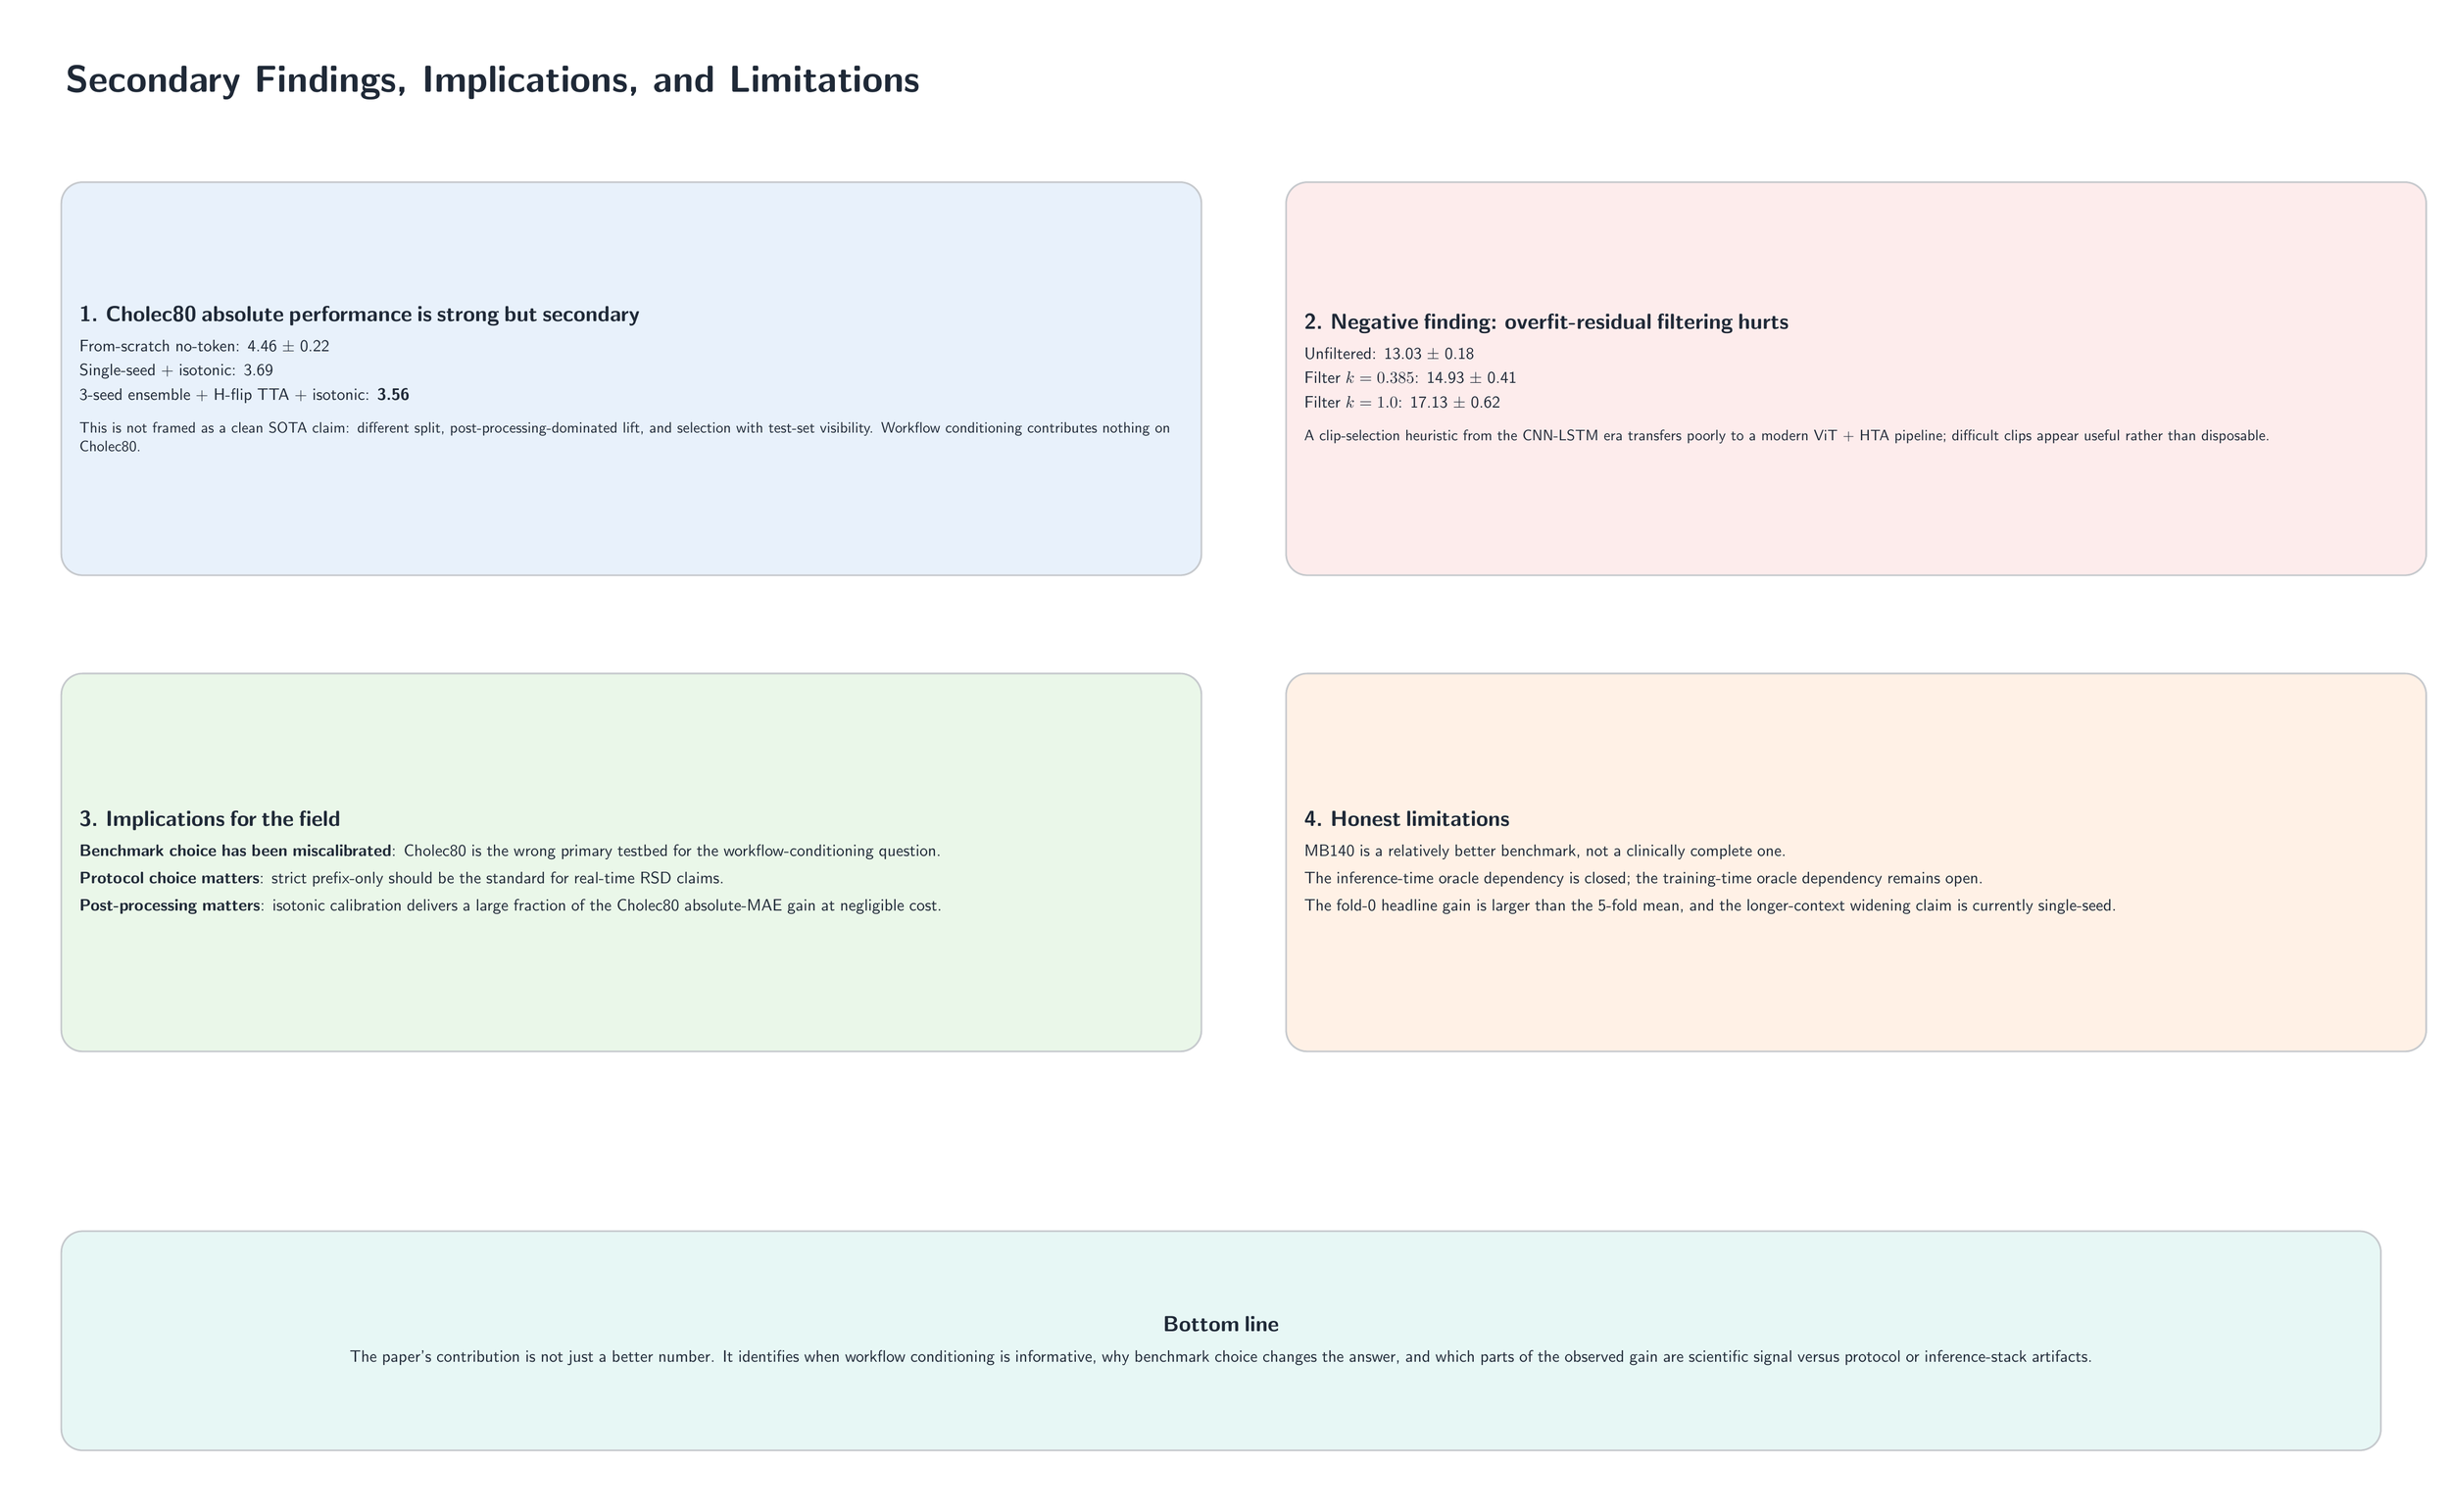
\begin{tikzpicture}[x=1pt,y=1pt]
\useasboundingbox (0,0) rectangle (1600,980);

\node[title, anchor=north west] at (30,950)
{Secondary Findings, Implications, and Limitations};

\node[bluebox, text width=730pt, minimum height=260pt, anchor=north west] at (30,870) {
{\subtitle 1. Cholec80 absolute performance is strong but secondary}\par\vspace{8pt}
{\body From-scratch no-token: 4.46 \(\pm\) 0.22}\par\vspace{4pt}
{\body Single-seed + isotonic: 3.69}\par\vspace{4pt}
{\body 3-seed ensemble + H-flip TTA + isotonic: \textbf{3.56}}\par\vspace{10pt}
{\smallbody This is not framed as a clean SOTA claim: different split, post-processing-dominated lift, and selection with test-set visibility. Workflow conditioning contributes nothing on Cholec80.}
};

\node[redbox, text width=730pt, minimum height=260pt, anchor=north west] at (840,870) {
{\subtitle 2. Negative finding: overfit-residual filtering hurts}\par\vspace{8pt}
{\body Unfiltered: 13.03 \(\pm\) 0.18}\par\vspace{4pt}
{\body Filter \(k=0.385\): 14.93 \(\pm\) 0.41}\par\vspace{4pt}
{\body Filter \(k=1.0\): 17.13 \(\pm\) 0.62}\par\vspace{10pt}
{\smallbody A clip-selection heuristic from the CNN-LSTM era transfers poorly to a modern ViT + HTA pipeline; difficult clips appear useful rather than disposable.}
};

\node[greenbox, text width=730pt, minimum height=250pt, anchor=north west] at (30,545) {
{\subtitle 3. Implications for the field}\par\vspace{8pt}
{\body \textbf{Benchmark choice has been miscalibrated}: Cholec80 is the wrong primary testbed for the workflow-conditioning question.}\par\vspace{6pt}
{\body \textbf{Protocol choice matters}: strict prefix-only should be the standard for real-time RSD claims.}\par\vspace{6pt}
{\body \textbf{Post-processing matters}: isotonic calibration delivers a large fraction of the Cholec80 absolute-MAE gain at negligible cost.}
};

\node[orangebox, text width=730pt, minimum height=250pt, anchor=north west] at (840,545) {
{\subtitle 4. Honest limitations}\par\vspace{8pt}
{\body MB140 is a relatively better benchmark, not a clinically complete one.}\par\vspace{6pt}
{\body The inference-time oracle dependency is closed; the training-time oracle dependency remains open.}\par\vspace{6pt}
{\body The fold-0 headline gain is larger than the 5-fold mean, and the longer-context widening claim is currently single-seed.}
};

\node[tealbox, text width=1510pt, minimum height=145pt, anchor=south west, align=center] at (30,30) {
{\subtitle Bottom line}\par\vspace{8pt}
{\body The paper's contribution is not just a better number. It identifies when workflow conditioning is informative, why benchmark choice changes the answer, and which parts of the observed gain are scientific signal versus protocol or inference-stack artifacts.}
};

\end{tikzpicture}
\end{document}
